\newpage
\section{Using \madanalysis\ and searching for dark matter (15/11/2016)}

\madanalysis\ is a tool used to perform analyses on phenomenological investigations (looking for new particles, new physics, excluding mass ranges of new particles, etc.) at particle colliders. It can analyse data generated by \madgraph\ and other Monte Carlo event generators. Simple analyses can be run using a Python interface (the "first running mode of the program"), whilst more complex analyses usually require the use of C++ (the "second running modes"). This is similar to ROOT; whilst it's easy and intuitive to use Python for simple scripts, C++ macros are normally needed for more complex stuff.

\textsc{MadAnalysis 5} \cite{Conte:2012madanalysis} can be downloaded in a tar ball from the Internet, with the requirements being listed in the README. It runs similarly to \textsc{MadGraph}: navigating to the directory \textbf{MadAnalysis/MA5\_v1\_4/} on my computer and typing \verb!./bin/ma5! runs the initialiser and dependency-checker. This environment is also where I can check for updates and install packages, just like in \madgraph\ (\verb!install <name of package>!, etc.). If I'm installing MadAnalysis for the first time, check which packages are already there, and install \textsc{Delphes} and other necessary ones. If a package won't install properly, try typing \verb!./bin/ma5 -R! and installing again. From now, until I state otherwise, I will be using \textsc{MadAnalysis 5} v1.4.

To run an analysis, type \verb!./bin/ma5  -s -R <name of input file>!, with the extension for the input file being .ma or .ma5. The \verb!-s! stands for "script mode" so the program quits after the script is executed, and the \verb!-R! stands for "reco", i.e., the program runs at the reconstructed level (by default, without \verb!-R!, it is launched at the parton level). When running at the reconstructed level, the package \textsc{FastJet} \cite{Cacciari:2011fastjet} is used, which is software for finding and analysing jets in collider data. An example of an input file -- which is a dark Higgs (Higgs-like particle that couples to dark matter) search -- is displayed below.

\lstinputlisting[language=Python, caption={A \madanalysis\ input file for a dark Higgs search based on the information in \cite{ATLAS-CONF-2016-019}. Output files from \madgraph\ can be imported to use as signal/background, cuts can be applied, and graphs can be plotted. File name: MonoDarkHiggs\_signal\_esh.ma (v1).}]{./sec13/MonoDarkHiggs_signal_eshv1.ma}

You import the signal/background files, apply cuts, plot graphs/histograms and get information (usually in the form of a \LaTeX\ document) out of it. The paper that this search is based on (that I \emph{need} to read) is \cite{ATLAS-CONF-2016-019}. A helpful, brief tutorial can be found at \url{https://madanalysis.irmp.ucl.ac.be/raw-attachment/wiki/Talks/FR2012_conte.pdf}.

As an example I ran an input file, importing \madgraph\ output files (\textbf{...\_pythia\_events.hep.gz}) from the runs I performed earlier in this document -- $pp \rightarrow t\bar{t}$, $pp \rightarrow W +$ jets, and $pp \rightarrow Z +$ jets -- as backgrounds to see how well the program worked and how output was handled. A \LaTeX\ document, displayed below, was produced containing the input, process details, and a histogram. Other output files (that can be used in other analyses) are also generated in the \textbf{$<$name of output$>$/Output/} directory.

\setboolean{@twoside}{false}
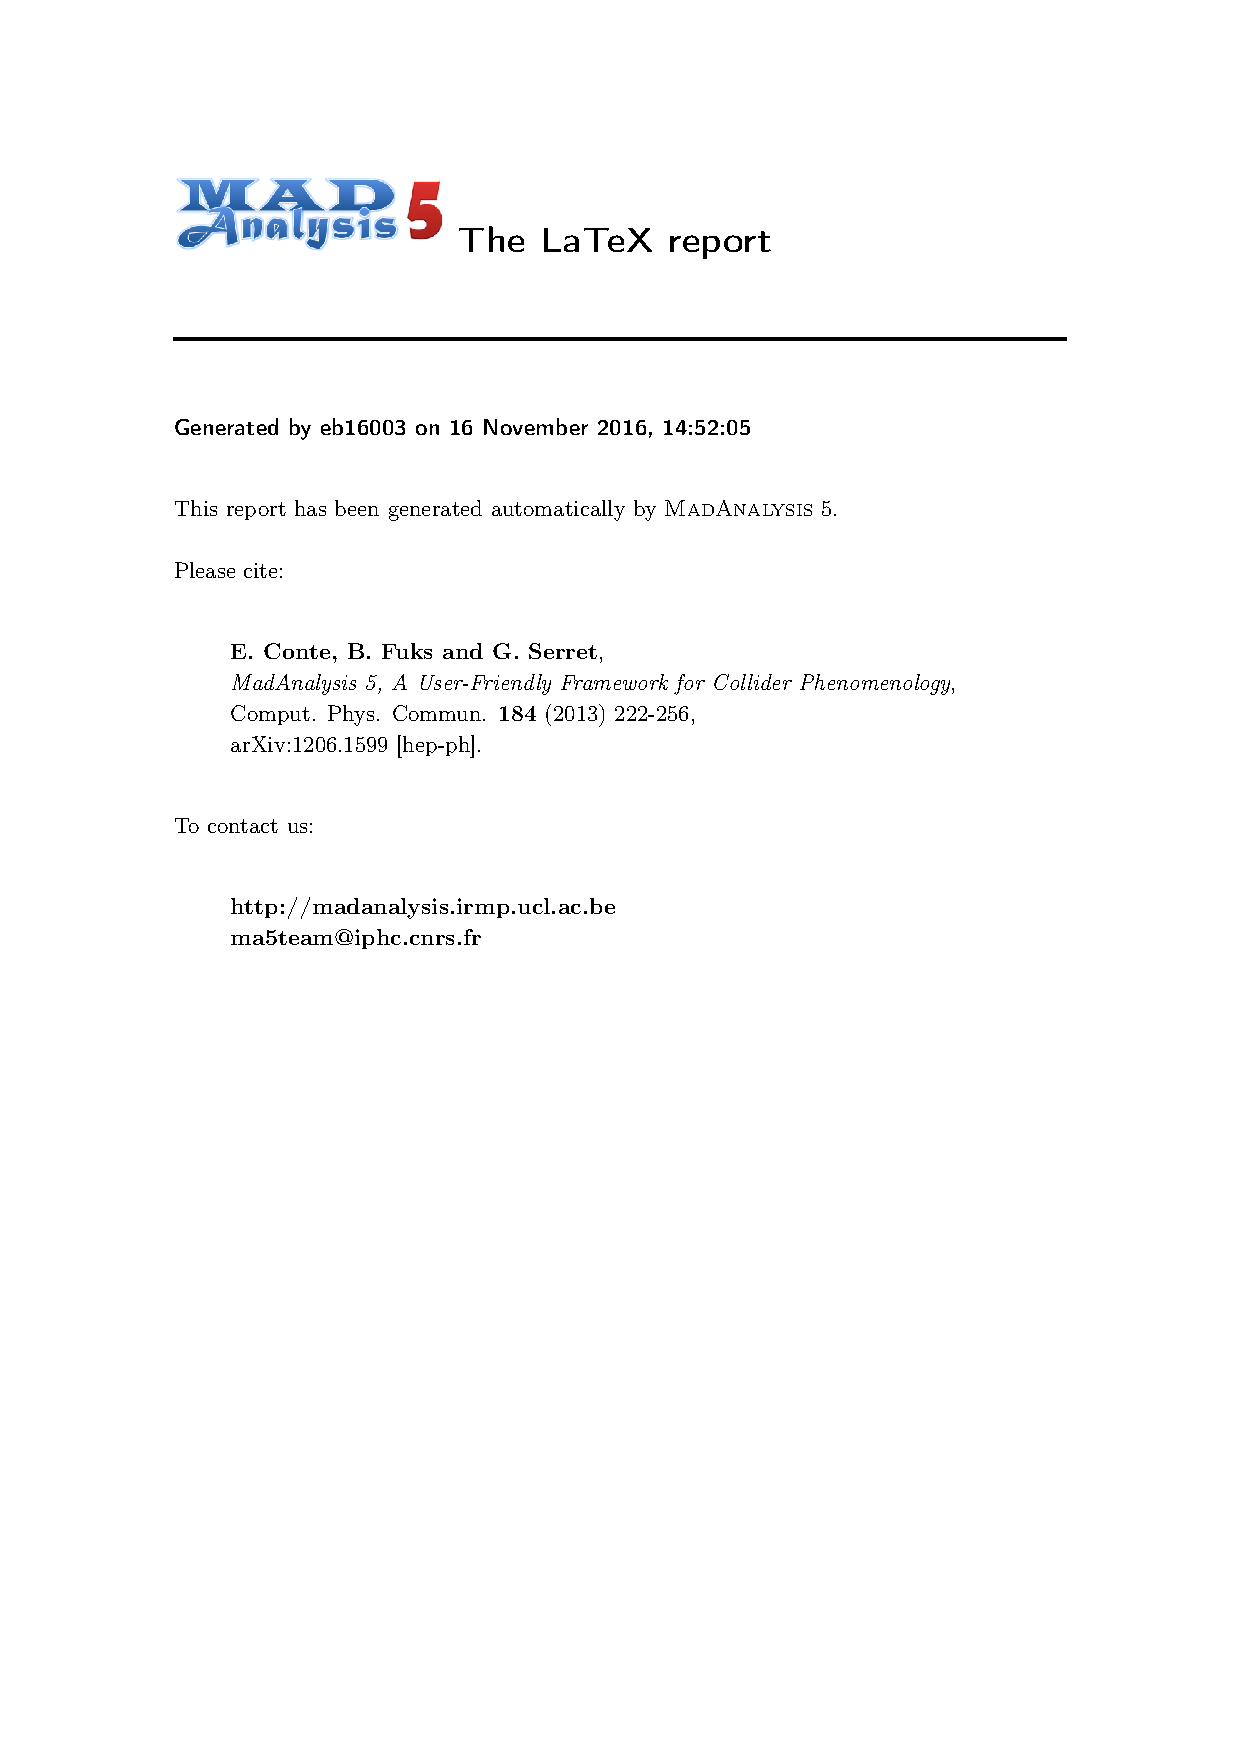
\includepdf[pages=-, offset=75 -75]{./sec13/mainv1.pdf}

The PDF (with the .tex and other \LaTeX\ files) is always generated in the directory \textbf{$<$name of output$>$/PDF/main.pdf}.

\textbf{As of now, this electronic version will serve as my main lab book. It's easier to type and edit on a computer than by hand, and it's much easier to include (versioned) code, figures and other inclusions this way, rather than printing them out and sticking them in. I may still write some stuff in my physical lab book but, to be honest, it's more of a hassle if I'm writing everything twice.}
